\documentclass{article}

\usepackage[spanish]{babel}
\usepackage[utf8]{inputenc}
\usepackage{hyperref}
\usepackage{graphicx}
\graphicspath{ {images/} }

\title{Inteligencia Artificial: Tema 1}

\author{Daniel Monjas Miguélez}

\date{\today}

\begin{document}
\maketitle

\newpage

\tableofcontents

\newpage

\section{Introducción}
Actualmente nos encontramos en la edad de hora de la Inteligencia Artificial, nunca se ha escrito, hablado e inveritdo tanto, ni la economía, ni la política, ni la sociedad han estado tan interesadas en la Inteligencia Artificial como actualmente. \\

Las grandes firmas TIC (Google, Apple, IBM, etc) están muy interesadas en el desarrollo y comercialización de productos con componentes inteligentes, lo que ha promovido la creación de puestos de trabajo en TIC que requieren conocimientos de IA y ha generado oportunidades de creación de empresas. Un ejemplo de esta última es DeepMind, una empresa de Inteligencia Artificial que fue absorbida por Google y que actualmente se encarga de grandes poryectos de IA. \\

En esta década pasada se ha realizado una inversión sin precedentes en la invertigación y desarrollo de IA. Se ha producido un crecimiento espectacular en los avances en la investigación en universidades, lo que ha dado lugar a la proliferación de startups basadas en IA. Las grandes firmas son conscientes de que la tecnología en IA está muy madura para poder desarrollar productos comerciales que satisfacen las necesidades de las personas. \\

La IA busca enconrar el algoritmo de la mente humana. Esta tiene una repercusión mediática y social sin precedentes.

\section{¿Qué significa ser inteligente?}
Es dificil definir inteligencia de una forma concreta. Según la R.A.E hay 7 definiciones diferentes:

\begin{enumerate}
\item Capacidad de entender o comprender.
\item Capacidad de resolver problemas.
\item Conocimiento, comprensión, acto de entender.
\item Sentido en que se puede tomar una sentencia, un dicho o una expresión
\item Habilidad, destreza y experiencia.
\item Trato y correspondencia secreta de dos o más personas o naciones entre sí.
\item Sustancia puramente espiritual.
\end{enumerate}

Según Howard Gardner la definición de inteligencia es,

\begin{itemize}
\item Capacidad de ordenar los pensamientos y coordinarlos con las acciones. La inteligencia no es una sola, sino que existen tipos distintos.
\end{itemize}

Gardner es conocido funamentalmente por su teoría de las inteligencias múltiples, que señala que no existe una inteligencia única en el ser humano, sino una diversidad de inteligencias que marcan los potenciales y acentos significativos de cada individuo, trazados por las fortalezas y debilidades en toda una serie de escenarios de expansión de la inteligencia. Gardner consideraba las siguientes inteligencias:

\begin{itemize}
\item \textbf{Inteligencia lingüistica.} 

\item \textbf{Inteligencia lógico-matemática.}

\item \textbf{Inteligencia corporal y cinética.}

\item \textbf{Inteligencia visual y especial.}

\item \textbf{Inteligencia musical.}

\item \textbf{Inteligencia interpersonal (inteligencia social).}

\item \textbf{Inteligencia intrapersonal.}

\item \textbf{Inteligencia naturalista.}
\end{itemize}

\section{¿Qué es inteligencia Artificial?}
En primer lugar, veremos definiciones sacadas de ocho libros de texto:

\begin{enumerate}
\item \label{top_1}``El excitante nuevo esfuerzo de hacer pensar a los ordenadores ... máquinas con mentes, en el sentido literal y completo.'' (Haugeland, 1985) \\

``La automatización de actividades que asociamos el pensamiento humano, actividades tales como toma de decisiones, resolución de problemas , aprender ...'' (Bellman, 1978)

\item \label{top_2} ``El estudio de facultades mentales a través del uso de modelos computacionale'' (Charniak y McDermott, 1985) \\

``El estudio de cálculo que hacen posible percibir, razonar, y actuar'' (Winston, 1992)

\item \label{top_3}``El arte de crear máquinas que realizan funciones que requieren inteligencia cuando son realizadas por persona'' (Kurzweil, 1990)  \\

 ``El estudio de como hacer que ordenadores realizen tareas en las cuales, por el momento, las personas son mejores'' (Rich y Knight, 1991)

\item \label{top_4} ``Un campo de estudio que busca explicar y emular comportamiento inteligente en términos de procesos computacionales'' (Schalkoff, 1990) \\

``La rama de las ciencias de la computación que se encarga de la automatización del comportamiento inteligente'' (Luger y Stubblefield, 1993).
\end{enumerate}

Estas ocho definiciones de Inteligencia Artificial están organizadas en :

\begin{enumerate}
\item Sistemas que piensan como humanos (modelos cognitivos).

\item Sistemas que piensan racionalmente (leyes del pensamiento).

\item Sistemas que actuan como humanos (test de Turing).

\item Sistemas que actuan racionalmente (agentes racionales).
\end{enumerate}

Históricamente se han seguido las cuatro aproximaciones. Como uno cabría esperar, existe tensión entre las aproximaciones centradas entorno a loas humanos y las aproximaciones centradas entorno al racioncinio. Las personas de cada grupo a veces muestran aprensión por el trabajo hecho por los otros grupos, pero en verdad cada dirección ha conseguido logros valiosos. \\

La inteligencia Artificial es una rama de la informática que estudia y resuelve problemas situados en la frontera de la misma. Se basa en dos ideas fundamentales, representación del conocimiento explícita y declarativa y resolución de problemas (heurística). \\

\textbf{¿Es la IA posible?} la posibilidad de inteligencia artificial plantea problemas filosóficos complejos.

\section{Sistemas que piensan como humanos: Aproximación del Test de Turing}
Las leyes del pensamiento racional se funamentan en la lógica. La lógica formal está en la base de los programas inteligentes, pero se presentan dos obstáculos:

\begin{enumerate}
\item Es muy difícil formalizar el conocimiento

\item Hay un gran salto entre la capacidad teórica de la lógica y su realización práctica.
\end{enumerate}

En este caso el modelo es el ser humano, el objetivo es construir un sistema que pase por humano. Surge así el test de Turing, un test en el que en teoría si es superado el sistema que lo supera es inteligente. La interacción de programas con personas hace que sea necesario que estos actúen como humanos. Surge de esta manera el test de Turing total.

\subsection{Test de Turing}
El test de Turing, propuesto por Alan Turing, fue diseñador para proveer una definición de inteligencia operacional satisfactoria. Turing definió comportamiento inteligente como la habilidad de conseguir rendimiento a nivel humano en todas las tareas cognitivas, suficiente para engañar a un interrogante. Para que un computador pase el test debe poseer:

\begin{itemize}
\item Procesamiento del lenguaje natural, para habilitar la comunicación satisfactoriamente.

\item Representación del conocimiento para almacenar información proveida antes o durante el interrogatorio.

\item Razonamiento automatizado para usar la información almacenada para responder preguntas y generar nuevas conclusiones.

\item Machine learning para adaptarse a nuevas circunstancias y detectar y extrapolar patrones.
\end{itemize}

El test de Turing deliberadamente esquiva la interacción física directa entre el interrogante y el ordenador, ya que la simulación física con una persona es innecesaria para la inteligencia. De todas forma, el test de Turing total incluye una señal de video de forma que el interrogante puede probar las habilidades perceptivas del sujeto. Para superar el test de Turing total, el computador necesitaría

\begin{itemize}
\item Visión por computador para percibir objetos

\item Robotica para moverlos
\end{itemize}

\section{Sistemas que actúan racionalmente}
Actuar racionalmente significa actuar de forma que se alcanza una meta, dados unas creencias. Un agente es solo algo que percibe y actua, siempre según el entorno en el que está situado. En esta aproximación, la Inteligencia Artificial es vista como el estudio y construcción de agentes relacionales. Un agente relacional actúa de la manera correcta según al información que poseea, actúa para alcanzar el mejor resultado o, con incertidumbre, el mejor resutlado esperado. \\

Hacer inferencias correctas es a veces parte de ser un agente relacional, porque una forma de actuar racionalmente es razonar logicamente hasta la conclusión de que una acción dada nos llevará a nuestra meta, y entonces actuar en consecuencia. Por otro lado, una inferencia correcta no es toda la racionalidad, porque a menudo se dan situaciones donde no hay nada probablemente correcto, aun así algo se tiene que hacer. \\

Todas las habilidades cognitivas requeridas para el test de Turing estan ahí para permitir acciones racionales. El estudio de Inteligencia Artificial como un agente racional tiene dos ventajas. La primera, es  que es más general que la aproximación de las leyes del pensamiento, puesto que la inferencia correcta es solo un mecanimso útil para obtener raciocinio, y no uno necesario. La segunda, es que es más ameno especificar el desarrollo que usar aproximaciones basadas en el pensamiento o el comportamiento humano, puesto que el raciocinio estandar es clarmente definido y completamente general. \\

\section{La habitación china de Searle}
En una habitación cerrada, con un orificio de entrada y uno de salida, se coloca a un sujeto con un diccionario chino. Cada vez que el sujeto recibe un documento en chino por la entrada, lo traduce y devuelve el documento resultante por la salida. \\

Para el que no conozca el sistema, este en su conjunto ``sabe chino'', pero ¿realmente el sujeto sabe chino?. La computación actual es usar reglas sintácticas para manipular cadenas de símbolos, sin comprender el significado o la semántica. El argumento es que no se puede alcanzar la inteligencia humana con el mero manejo de símbolos.

\section{Bases de la inteligencia artificial - Filosofía}

\begin{figure}[h]
\centering
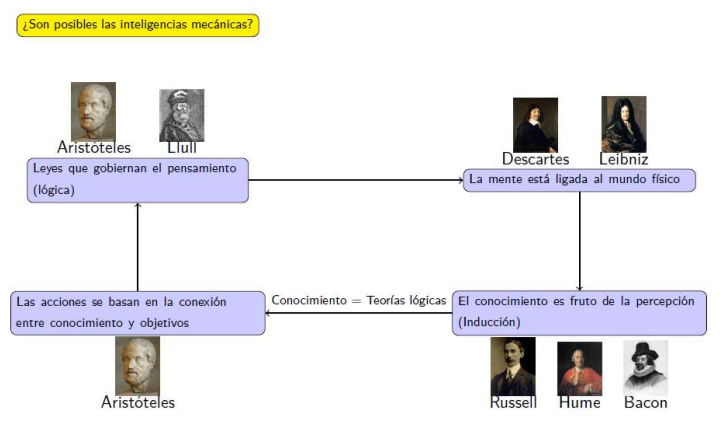
\includegraphics[scale=1,width=1\textwidth]{esquema_historia.png}
\end{figure}

\begin{figure}
\centering
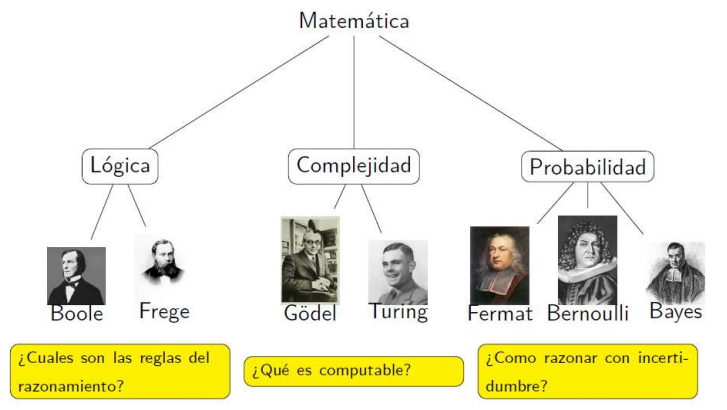
\includegraphics[scale=1,width=0.8\textwidth]{bases_ia.png}
\end{figure}

\begin{itemize}
\item \textbf{Economía:} En el ámbito de la economía surge la teoría de la decisión, teoría de juegos, investigación operativa, etc.

\item \textbf{Neurociencia:} neuronas/especialización del cerebro.

\item \textbf{Psicología:} psicología cognitiva/ciencias cognitivas: teorías sobre la conducta, bases del comportamiento racional.

\item \textbf{Computación:} para la existencia de la IA es necesario un mecanismo para soportarlo. También son necesarias las herramientas para desarrollar programas de IA.

\item \textbf{Teoría de control/cibernética:} construcción de sistemas autónomos.

\item \textbf{Lingüística:} Chomsky, representación del conocimiento, gramática de la lengua. Lingüística computacional.
\end{itemize}

\section{Historia de la IA}
Como disciplina, IA ha pasado por las siguientes fases:

\begin{itemize}
\item \textbf{Período de gestación (1943-1955):} se desarrollan los primeros modelos neuronales artificailes que simulan una neurona biológica (McCulloch y Pitts, 1943). Test de Turing (1950). IA en Juegos (Damas 1951). Logic Theorist (1955).

\item \textbf{Nacimiento (1956):} conferencia Dartmouth, se perfila la disciplina \textbf{Inteligencia Artificial}, cuyo objetivo es duplicar facultades humanas como creatividad, automejora, uso del lenguajes, etc.

\item \textbf{Años dorados (1956-1974):} Razonamiento como búsqueda. General Problem Solver, hipótesis de sistema de símbolos físicos, Geometry Problem Solver, Advice Takes, mundo de los bloques, etc. Procesamiento Lenguaje Natural. ``Micro mundos''. Optimismo exacerbado. Inversión notables (DARP, MIT, CMU, SRAI,Edinburgh University)...

\item \textbf{Sistemas Basados en el conocimiento (1969-1974):} se desarrollan los primeros sistemas expertos (DRENDAL para reconocer moléculas, MYCIN para diagnóstico médico, SHRDLU para entender el lenguaje natural, desarrollo de LISP y Prolog, etc.)

\item \textbf{Primer invierno:1974-1980}

\begin{itemize}
\item \textbf{Edad oscura (1966-1973):} potencia muy limitada de cómputo. Se encuentran dificultades debido al gran conocimiento general necesario para resolver problemas específicos (conocimiento de sentido común) y la intratabilidad, explosión combinatoria, de algunos problemas. Paradoja de Moravec. Comparativamente es fácil conseguir que las computadoras muestren capacidades similares a las de un humano adulto en tests de inteligencia, y difícil o imposible lograr que posean las habilidades perceptivas y motrices de un bebé de un año.

\item \textbf{Fin de la financiación} (los objetivos eran ``demasiado grandiosos''). Críticas de otros campos (Searle, a ELIZA).

\item \textbf{Edad oscura del conexionismo} y aparición de Lisp y Prolog como paradigmas de programación lógica y simbólica.
\end{itemize}

\item \textbf{Boom IA en la industria (1980-1987):} sistemas expertos y la revolución de la ingeniería del conocimiento. (Control difuso, diseño de chips, interfaces hombre-máquina, algoritmos heurísticos, resolución de problemas de logística, etc.). Vuelve la financiación.

\item \textbf{Nueva era de las redes neuronales artificiales (1986-...):} se empiezan a considerar las RR.NN como herramientas de ingeniería capaz de modelar datos y comportamientos deseados en sistemas físicos.

\item \textbf{Fracaso: el segundo invierno (1987-1993)}

\begin{itemize}
\item \textbf{Colapso del hardware especializado en IA.} El éxito del PC destruyó las esperanzas de las ``máquinas Lisp''. Los sistemas expertos eran muy caros de mantener.

\item \textbf{La importancia de tener un cuerpo. Pensamiento dominante:} la robótica era la base de la IA y no al revés.
\end{itemize}

\item \textbf{Resurgimiento (1993-2011)}

\begin{itemize}
\item \textbf{Grandes hitos.} La ley de Moore: Deep blue($x10^6$ veces más rápido que el primer programa de damas), DARPA challenges (Grand, Urban). Watson gana Jeopardy! (Watson fue un ordenador IBM que ganó el concurso Jeopardy, un show de televisión).

\item \textbf{IA como ciencia (1987-actualidad):} la gran cantidad de investigación y sistema de IA desarrollados son, en sí mismos, objeto de estudio independiente de las áreas de las que surgió. Surgen disciplinas como data mining, tecnologías de agentes, metaheurísticas, algoritmos basados en procesos biológicos, etc.

\item \textbf{Emergen los Agentes inteligentes: la IA es el estudio de los agentes inteligentes.} SOAR (arquitectura cognitiva) ejemplo de un ``agente total'', con distintos tipos de capacidades cognitivas (percibir, razonar, actuar, aprender, ...), pero integradas en una misma arquitectura.

\item \textbf{IA detrás de todo:} Softbots, bots, agentes de internet, motores de búsqueda, sistemas recomendadores, agregadores de páginas web.
\end{itemize}

\item \textbf{2011-actualidad}

\begin{itemize}
\item \textbf{BigData.} Cantidades masivas de datos generados cada día, solo pueden ser analizados por algoritmos necesariamente inteligentes (descripción, predicción, prescripción)

\item \textbf{Deep Learning.} Arquitecturas de cómputo paralelas (GPUs) han acelerado las capacidades de las Redes Neuronales.

\item \textbf{IA General.} Encontrar un algoritmo que actúe y aprenda en cualquier entorno.
\end{itemize}

\end{itemize}



\end{document}